\documentclass[11pt]{article}
\usepackage{deauthor}
\usepackage{times}
\usepackage{soul}
\usepackage{wrapfig}
\usepackage{graphicx}
\usepackage{xspace}
\usepackage[it,small]{caption}
\usepackage[export]{adjustbox}

\usepackage{cite}
\usepackage{amsmath,amssymb,amsfonts}
\usepackage{textcomp}
\usepackage{graphicx} 
\usepackage{algorithm}    
\usepackage{algorithmic} 
\usepackage{xcolor} 


% ensure times
\usepackage{txfonts}
\usepackage{url}

\usepackage{balance}  % for  \balance command ON LAST PAGE  (only there!)
\usepackage{booktabs} % For formal tables
\usepackage{enumitem}
\usepackage{multirow}
\usepackage{subfigure}

\usepackage[pdfpagelabels=false]{hyperref}

\usepackage{listings}

\usepackage{mathtools}
\DeclarePairedDelimiter\ceil{\lceil}{\rceil}
\DeclarePairedDelimiter\floor{\lfloor}{\rfloor}

% -- Cypher
\lstset{ %
  language=SQL,                % choose the language of the code
  basicstyle=\ttfamily\footnotesize,     % the size of the fonts that are used for the code
  %numbers=left,                   % where to put the line-numbers
  %numberstyle=\small,             % the size of the fonts that are used for the line-numbers
  %stepnumber=1,                   % the step between two line-numbers. If it is 1 each line will be numbered
  %numbersep=3pt,                  % how far the line-numbers are from the code
  backgroundcolor=\color[rgb]{0.92,0.92,0.92},  % choose the background color. You must add \usepackage{color}
  showspaces=false,               % show spaces adding particular underscores
  showstringspaces=false,         % underline spaces within strings
  showtabs=false,                 % show tabs within strings adding particular underscores
  %frame=tb,                       % adds a frame around the code
  tabsize=2,                      % sets default tabsize to 2 spaces
  captionpos=b,                   % sets the caption-position to bottom
  breaklines=true,                % sets automatic line breaking
  breakatwhitespace=false,        % sets if automatic breaks should only happen at whitespace
  keywordstyle=\color{blue},      % define style for keywords
  commentstyle=\color{ForestGreen},      % define style for comment
  stringstyle=\color{gray},       % define style for strings
  escapeinside={\%*}{*)},         % use a latex within your code
  morekeywords={id, return, with}, 
  deletekeywords={concat, input, output},
  emph={                          % emphersize group for user defined functions
    0, 1, 30, 31
  },
  emphstyle={\color{red}}%, %\bfseries}%\scshape
  %emph={[2]                       % emphersize group for system set functions
  %  CONCAT, ID, UNION, INTERSECT, COUNT, SPLIT
  %},
  %emphstyle={[2]\color{BurntOrange}}
}

\renewcommand*{\lstlistingname}{\small{Query}}


% shortcuts
\newcommand{\provdb}{{\sc ProvDB}\xspace}
\newcommand{\prov}{{\sc PROV}\xspace}
\newcommand{\eat}[1]{}
\newcommand{\cmd}[1]{{\tt #1}}
\newcommand{\topic}[1]{\vspace{3pt}\noindent\underline{\bf #1}}
\newcommand{\tighttopic}[1]{\vspace{-0.30pt}\noindent\underline{\bf #1}}
\newcommand{\subtopic}[1]{\noindent{{\small\textbf{\emph{ #1}}}}}


\newcommand{\tlp}[1]{} 
\newcommand{\tnote}[1]{} 

\newcommand{\opseg}{{\sc PgSeg}\xspace}
\newcommand{\opsum}{{\sc PgSum}\xspace}

% opseg notations
\newcommand{\vertexset}{$\mathbb V$}
\newcommand{\edgeset}{$\mathbb E$}

\newcommand{\entity}{$\mathcal E$}
\newcommand{\activity}{$\mathcal A$}
\newcommand{\agent}{$\mathcal U$}
\newcommand{\used}{$\mathit U$}
\newcommand{\wasGeneratedBy}{$\mathit G$}
\newcommand{\wasAssociatedWith}{$\mathit S$}
\newcommand{\wasAttributedTo}{$\mathit A$}
\newcommand{\wasDerivedFrom}{$\mathit D$}

\newcommand{\inv}[1]{#1\raisebox{1.15ex}{$\scriptscriptstyle-\!1$}}
\newcommand{\usedInv}{\inv{\used}}
\newcommand{\wasGeneratedByInv}{\inv{\wasGeneratedBy}}

\newcommand{\vlabelfunc}{$\lambda_v$}
\newcommand{\elabelfunc}{$\lambda_e$}
\newcommand{\property}{$\mathcal P$}
\newcommand{\vpropfunc}{$\sigma$}
\newcommand{\epropfunc}{$\omega$}
\newcommand{\provgraph}{$\mathcal G$}

% segmentation concepts
\newcommand{\interestedSnapshots}{$\mathcal Q_E$}
\newcommand{\segSource}{{\footnotesize{$\mathcal V_{src}$}}}
\newcommand{\segDestination}{{\footnotesize{$\mathcal V_{dst}$}}}
\newcommand{\segInduced}{{\footnotesize{$\mathcal V_{ind}$}}}
\newcommand{\segInducedOnPath}{{\footnotesize{$\mathcal V^{C_1}_{ind}$}}}
\newcommand{\segInducedSimilarPath}{{\footnotesize{$\mathcal V^{C_2}_{ind}$}}}
\newcommand{\segInducedGenTogether}{{\footnotesize{$\mathcal V^{C_3}_{ind}$}}}
\newcommand{\segInducedAgents}{{\footnotesize{$\mathcal V^{C_4}_{ind}$}}}

\newcommand{\similarPathPatternRule}{{\sc{SimProv}}}
\newcommand{\genTogetherPathPatternRule}{{\sc{GenTogether}}}

\newcommand{\opsegAlg}{{\sc{SimProvAlg}}}
\newcommand{\opsegAlgTst}{{\sc{SimProvTst}}}
%\newcommand{\opsegAlg}{{\sc{SpvAlg}}}
%\newcommand{\opsegAlgTst}{{\sc{SpvTst}}}
\newcommand{\baselineAlg}{{\sc{CflrB}}}

%\newcommand{\similarProvPathRule}{{\sc{SimProvPathSeg}}}

\newcommand{\cfglanguage}[1]{{\small{$L(\text{#1})$}}}

\newcommand{\boundaryCriteria}{{\small{$\mathcal B$}}}
\newcommand{\actualLabel}{$\mathcal F$}
\newcommand{\segsubgraph}{$\mathcal S$}
\newcommand{\segv}{$\text{\vertexset}_{\text{\segsubgraph}}$}
\newcommand{\sege}{$\text{\edgeset}_{\text{\segsubgraph}}$}
\newcommand{\segsubgraphFull}{$\text{\segsubgraph}(\text{\segv},\text{\sege})$}
\newcommand{\segsubgraphFullWithI}{$\text{\segsubgraph}_i(\text{\segv}_i,\text{\sege}_i)$}

\newcommand{\pathlabel}{$\tau$}
\newcommand{\pathlabelword}[1]{{\small{#1}}}

\newcommand{\segpathshort}{$\pi$}
\newcommand{\segsubpathshort}{$\hat\pi$}
\newcommand{\segpath}[2]{$\pi_{\text{#1},\text{#2}}$}
\newcommand{\segsubpath}[2]{$\hat\pi_{\text{#1},\text{#2}}$}

% opsum notations
\newcommand{\opsumgraph}{{\sc Psg}}
\newcommand{\psgvertex}{{\mathcal M}}
\newcommand{\psgedge}{E}
\newcommand{\psgvpropfunc}{\rho}
\newcommand{\psgepropfunc}{\gamma}
\newcommand{\propagg}{$\mathcal K$}
\newcommand{\propaggtyped}[1]{${\small{\text{\propagg}}}_\text{#1}$}
\newcommand{\vertexeqrel}{$\equiv^k_{\kappa}$}
\newcommand{\vertexeqrelpartition}{$P^{\text{\vertexeqrel}}$}
\newcommand{\provtype}{$\mathcal R$}
\newcommand{\provtypehop}[1]{$\text{\provtype}_{#1}$}
\newcommand{\segmentset}{$\mathbb S$}
\newcommand{\segmentsetallv}{$\mathbb V_{\text{\segmentset}}$}
\newcommand{\segmentsetalle}{$\mathbb E_{\text{\segmentset}}$}
\newcommand{\sumpathshort}{$\pi$}
\newcommand{\sumpath}[2]{$\text{\sumpathshort}_{#1,#2}$}


% writeup marker
\newcommand{\todo}[1]{{\color{blue}{\textbf{TODO}: #1}}}
\newcommand{\goal}[1]{{\color{green}{\textbf{Goal}: #1}}}
\newcommand{\refpaper}[1]{{\color{orange}{\textbf{Ref paper}: #1}}}
\newcommand{\sketch}[1]{{\color{gray}{\scriptsize{#1}}}}
\newcommand{\outline}[1]{{\sc \color{purple}{\% #1}\\}}
\newcommand{\workline}[1]{\hl{\quad\quad\quad\quad\quad\quad #1 \quad\quad\quad\quad\quad\quad\\}}

\newcommand{\pomo}{{\sc \color{red}{Op}}}

% datasets and evaluations
\newcommand{\syntheticpg}{{\sc Pd}}
\newcommand{\syntheticsg}{{\sc Sd}}

\newcommand{\intracedominant}{$\leq^t_{in}$}
\newcommand{\outtracedominant}{$\leq^t_{out}$}
\newcommand{\intraceequal}{$\simeq^t_{in}$}
\newcommand{\outtraceequal}{$\simeq^t_{out}$}

\newcommand{\insimulate}{$\leq^s_{in}$}
\newcommand{\outsimulate}{$\leq^s_{out}$}
\newcommand{\insimulationeq}{$\simeq^s_{in}$}
\newcommand{\outsimulationeq}{$\simeq^s_{out}$}

\newcommand{\sumbaseline}{{\tt pSum}}
\newcommand{\opsumAlg}{{\sc{PgSumAlg}}}

% for tune intro
\newcommand{\modelhub}{{\sc ModelHub}}

% reduce space
\newcommand{\lowPriority}[1]{} 
%\newcommand{\lowPriority}[1]{{\color{orange}{#1}}} 

\newcommand{\addedConent}[1]{#1}
%\newcommand{\addedConent}[1]{{\color{blue}{#1}}} 

% \newcommand{\introdrop}[1]{{\color{blue}{#1}}}
\newcommand{\abstractdrop}[1]{}
\newcommand{\introdrop}[1]{}
\newcommand{\segdrop}[1]{}
\newcommand{\sumdrop}[1]{}
\newcommand{\expdrop}[1]{}

\newcommand{\dhub}{{\sc Data\-Hub}\xspace}
\newcommand{\datahub}{\dhub}

\newcommand{\nosub}[1]{#1}
\newcommand{\nosubcite}[1]{}

\newcommand{\git}{{\tt git}\xspace}

\newcommand{\sourcegraph}{{correspondence graph}\xspace}

\newenvironment{longlist}{\setlength{\parindent}{0cm} \setlength{\parskip}{0.05cm}}{}

\title{ProvDB: Provenance-enabled Lifecycle Management of Collaborative Data Analysis Workflows}

\author{
Hui Miao,~ Amol Deshpande\\
       {University of Maryland, College Park, MD, USA}\\
       {{\large{\{}}hui,~amol{\large{\}}}@cs.umd.edu} 
}

\begin{document}

\maketitle

\begin{abstract}
Collaborative data science activities are becoming pervasive in a variety of communities, and are often conducted in teams, with people of different expertise performing back-and-forth modeling and analysis on time-evolving datasets. Current data science systems mainly focus on specific steps in the process such as training machine learning models, scaling to large data volumes, or serving the data or the models, while the issues of end-to-end data science lifecycle management are largely ignored. Such issues include, for example, tracking provenance and derivation history of models, identifying data processing pipelines and keeping track of their evolution, analyzing unexpected behaviors and monitoring the project health, and providing the ability to reason about specific analysis results. 
In this article, we present an overview of a unified provenance and metadata management system, called \provdb, that we have been building to support lifecycle management of complex collaborative data science workflows. 
\provdb captures a large amount of fine-grained information about the analysis processes and {\em versioned} data artifacts in a semi-passive manner using a flexible
and extensible ingestion mechanism; provides novel querying and analysis capabilities for simplifying bookkeeping and debugging tasks for data analysts; and enables a rich new set of capabilities like identifying flaws in the data science process. 
\end{abstract}




\section{Introduction}
Over the last two decades, we have seen a tremendous increase in collaborative
data science activities, where teams of data engineers, data scientists, and
domain experts work together to analyze and extract value from increasingly
large volumes of data. This has led to much work in industry and academia on
developing a wide range of tools and techniques, including  big data platforms,
data preparation and wrangling tools, new and sophisticated machine learning
techniques, and new environments like Jupyter Notebooks targeted at data
scientists. However, the widespread use of data science has also exposed the
shortcomings of the overall ecosystem, and has brought to the forefront a number
of critical concerns about how data is collected and processed, and how insights
or results are obtained from those. There are numerous examples of biased and
unfair decisions made by widely used data science pipelines, that are often
traced back to flaws in the training data, or mistakes or assumptions made
somewhere in the process of constructing those pipelines. Data analysis
processes are relatively easy to ``hack'' today, increasingly resulting in a
general lack of trust in published results (``fake news'') and many incidents of
unreproducible and/or retracted results.
\newpage

Addressing these concerns requires a holistic approach to conducting, auditing,
and continuously monitoring collaborative data science projects.  This however
is very challenging, because of the fundamentally ad hoc nature of collaborative
data science. It typically features highly unstructured and noisy datasets that
need to be cleaned and wrangled; amalgamation of different platforms, tools, and
techniques; significant back-and-forth among the members of a team; and
trial-and-error to identify the right analysis tools, algorithms, machine
learning models, and parameters. The data science pipelines are often spread
across a collection of analysis scripts, possibly across different systems.
Metadata or provenance information about how datasets were generated, including
the programs or scripts used for generating them and/or values of any crucial
parameters, is often lost.  As most datasets and analysis scripts evolve over
time, there is also a need to keep track of their {\em versions} over time;
using version control systems (VCS) like {\em git} can help to some extent, but
those don't provide sufficiently rich introspection capabilities.  

Lacking systematic platforms to support collaborative data science, we see users
manually track and act upon such information.  For example, users often manually
keep track of which derived datasets need to be updated when a source dataset
changes; they use spreadsheets to list which parameter combinations have been
tried out during the development of a machine learning model; and so on. This is
however tedious and error-prone, requires significant discipline from the users,
and typically lacks sufficient coverage.


In this article, we present an overview of our \provdb system, for unified
management of all kinds of metadata about collaborative data science workflows
that gets generated during the analysis processes. \provdb is being developed
under the umbrella of the {\bf DataHub} project~\cite{datahub2015}, where our
overarching goal is to understand and investigate the major pain points for data
engineers and scientists today, and develop tools and techniques for managing a
large number of datasets, their versions over time, and derived data products
and for supporting the end-to-end data science lifecycle. \provdb is designed to
be a standalone system, with complementary functionality to dataset versioning
tools developed
in~\cite{dataset2015,decibel,modelhub@icde17,dex@sigmod17,rstore}. Specifically,
\provdb manages and enables querying information about:
\textbf{(a)} version lineages of data, scripts, and results (collectively called {\em artifacts}),
\textbf{(b)} data provenance among artifacts which may or may not be structured, and
\textbf{(c)} workflow metadata on derivations and dependencies among artifact
snapshots, and \textbf{(d)} other context metadata that may be collected (e.g., summary logs).
By making it easy to mine and query this information in a unified fashion,
\provdb enables a rich set of functionality to simplify the lives of data
scientists, to make it easier to identify and eliminate errors, and to decrease
the time to obtain actionable insights.

To accommodate the wide variety of expected use cases, \provdb adopts a
``schema-later'' approach, where a small base schema is fixed, but users can add arbitrary semistructured information (in JSON) for recording additional metadata. 
The specific data model we use generalizes the standard W3C \prov\ data model, extended to allow flexibly capturing a variety of different types of information including versioning and provenance
information, parameters used during experiments or modeling, statistics gathered to make decision, analysis scripts, and notes or tags.
We map this logical data model to a {\em property graph data model}, and use the Neo4j graph database to store the information. 

\provdb features a suite of extensible {\em provenance ingestion} mechanisms. The currently supported ingestors are targeted at users who conduct the data
analysis using either {\tt UNIX Shell} or {\tt Jupyter Notebooks}. In the former case, user-run {\tt shell} commands to manipulate files or datasets are intercepted, and 
the before- and after-state of the artifacts is analyzed to generate rich metadata. Several such ingestors are already supported and new ingestors can be easily 
registered for specific commands. For example, such an ingestion program is used to analyze log files generated by Caffe (a deep learning framework) and to generate metadata 
about accuracy and loss metrics (for learned models) in a fine-grained manner. \provdb also features APIs to make it easy to add provenance or context information from other 
sources.

Finally, \provdb features many different mechanisms for querying and analyzing
the captured data. In addition to being able to use the querying features of
{\tt Neo4j} (including the Cypher and Gremlin query languages), \provdb also
features two novel graph query operators, {\em graph segmentation} and {\em
graph summarization}, that are geared towards the unique characteristics of
provenance information. 

\section{ProvDB Architecture}
\label{sec:sys_arch}

\provdb is a stand-alone system, designed to be used in conjunction with a
dataset version control system (DVCS) like {\tt git} or {\tt
DataHub}~\cite{datahub2015,provenance2015,dex@sigmod17,dataset2015} (Figure
\ref{fig:sys_arch}). The DVCS will handle the actual version management tasks,
and the distributed and decentralized management of individual {\em
repositories}.  A repository consists of a set of {\em versions}, each of which
is comprised of a set {\em artifacts} (scripts, datasets, derived results,
etc.). A version, identified by an ID, is \ul{immutable} and any update to a
version conceptually results in a new version with a different version ID
(physical data structures are typically not immutable and the underlying DVCS
may use various strategies for compact storage~\cite{dataset2015}). New versions
can  also be created through the application of transformation programs to one
or more existing versions.  We assume the DVCS supports standard version control
operations including {\sc checkout} a version, {\sc commit} a new version,
create a {\sc branch}, {\sc merge} versions, etc. 

\begin{wrapfigure}{r}{4.4in}
\centering{\mbox{\ \ }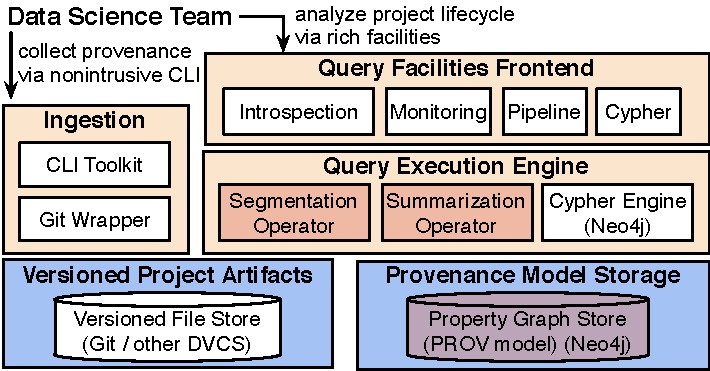
\includegraphics[width=0.62\textwidth]{figs/sys_arch.pdf}}
\caption{Architecture Overview of \provdb}
\label{fig:sys_arch}
\end{wrapfigure}

Most of the \provdb modules are agnostic to the DVCS being used, as long as
appropriate pipelines to transfer versioning metadata and context data are set
up.  The current implementation is based on {\tt \bfseries git}, in which case,
the repository contents are available as files for the users to operate upon;
the users can run whichever analysis tools they want on those after checking
them out, including distributed toolkits like Hadoop or Spark. 



Broadly speaking, the data maintained across the system can be categorized into: 
\begin{itemize}
\item[(a)] raw data that the users can directly access and analyze including the datasets, analysis scripts, and any derived artifacts such as trained models, and 
\item[(b)] metadata or provenance information transparently maintained by the system, and used for answering queries over the versioning or provenance information. 
\end{itemize}
Fine-grained record-level provenance information may or may not be directly accessible to the users depending on the ingest mechanism used. Note that, the split design that we have chosen to pursue requires duplication of some information in the DVCS and \provdb. We believe this is a small price to pay for the benefits of having a standalone provenance management system.

{\bf \provdb Ingestion module} is a thin layer on top of the DVCS (in our case, \git) that is used to capture the provenance and metadata information. This layer needs
to support a variety of functionality to make it easy to collect a large amount of metadata and provenance information, with minimal overhead to the user
(Sec.~\ref{sec:ingestion}). The \provdb instance itself is a separate process, and currently uses the Neo4j graph database for {\bf provenance model storage}; we chose Neo4j because of its support for the flexible property graph data model, and graph querying functionality out-of-the-box (Sec. \ref{sec:model}). 
The data stored inside \provdb can be queried using Cypher through the Neo4j frontend; \provdb\ {\bf query execution engine} also supports two novel types of {\em
segmentation} and {\em summarization} queries that we breifly describe in Section~\ref{sec:query}. Richer queries can be supported on top of these low-level querying
constructs; \provdb currently supports a simple form of continuous monitoring query, and also has a visual frontend to support a variety of provenance queries (Section~\ref{sec:query}).

\begin{figure*}[t!]
\centering{
\subfigure[An Example for a Data Science Project Lifecycle \& Associated Provenance]{
  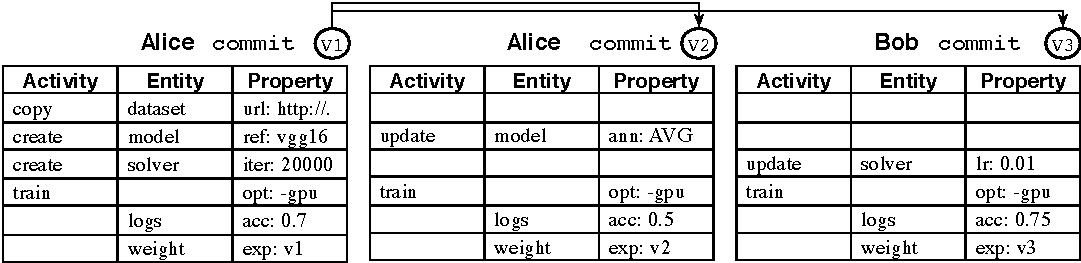
\includegraphics[width=0.645\textwidth]{figs/lifecycle_example.pdf}
  \label{fig:example_lifecycle}
}
\subfigure[Illustration of the W3C \prov\ Data Model]{
  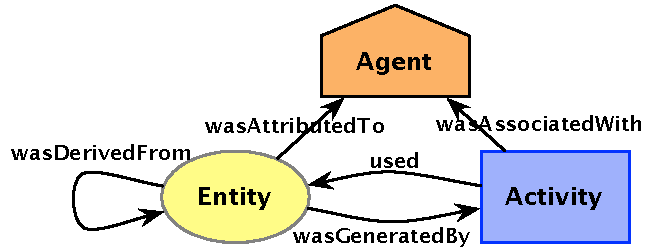
\includegraphics[width=0.32\textwidth,trim=0 0 0 10]{figs/standard_prov_concepts.pdf}
  \label{fig:prov}
}
\\\vspace{-3.2pt}
\subfigure[Provenance Graph for the Lifecycle Example (Some edges and properties are not shown due to space constraints)]{
  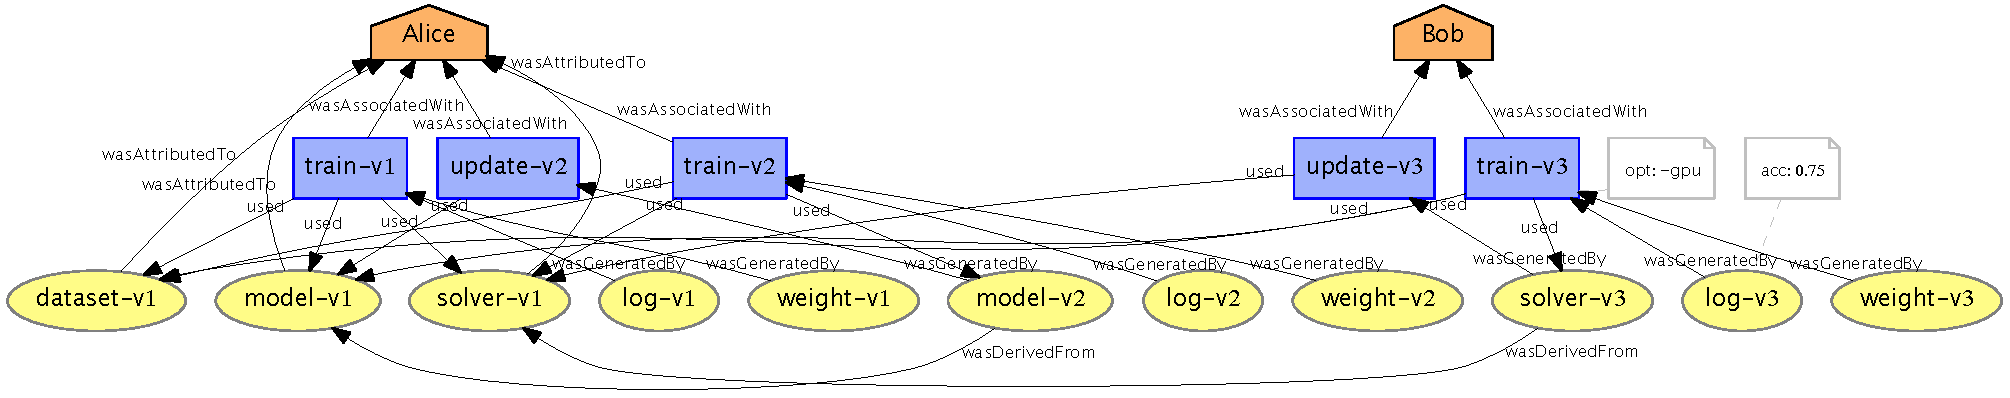
\includegraphics[width=1.0\textwidth,trim=0 0 0 12]{figs/example_prov_model.pdf}
  \label{fig:example_provenance}
}
}
\vspace{-7pt}
\caption{Illustration of Provenance Data Model and Query Operators in Data Science Lifecycles}
\vspace{-12pt}
\label{fig:example}
\end{figure*}



\section{Provenance Data Model and Provenance Graphs}
\label{sec:model}
The ingested provenance over the lifecycle of a data science project naturally forms a directed acyclic graph\footnote{We use versioning to avoid cyclic
self-derivations of the same entity and overwritten entity generations by some activity.}, combining heterogeneous information including a version graph representing the artifact changes, a workflow graph reflecting the derivations of those artifact versions, and a conceptual model graph showing the involvement of problem solving methods in the project~\cite{ground@cidr17,provdb@hilda17}. 
To represent the provenance graph and keep our discussion general to other provenance systems, after originally using a custom model, we switched to using the W3C \prov\ data model~\cite{prov_dm@w3c_tr13}, which is a standard interchange model for different provenance systems. 
We use the core set of \prov\ data model shown in Fig.~\ref{fig:prov}. 
There are three types of vertices (\vertexset) in the provenance graph in our context:
\begin{enumerate}[leftmargin=18pt,label=\emph{\alph*})]{}
\item 
\ul{Entities} (\entity) are the project artifacts (e.g., files, datasets, scripts) which the users work on and talk about; 
\item
\ul{Activities} (\activity) are the system or user actions (e.g., \cmd{train}, \cmd{git commit}, \cmd{cron} jobs) which act upon or with entities over a period of time, $[t_i, t_j)$; 
\item
\ul{Agents} (\agent) are the parties who are responsible for some activity (e.g., a team member, a system component). 
\end{enumerate}
Among the vertices, there are five types of directed edges (\edgeset): 
\begin{enumerate}[leftmargin=18pt,label={\roman*})]{}
\item    
An activity started at time $t_i$ often uses some entities (\ul{`used'}, \used $\subseteq$ \activity $\times$ \entity);  
\item
then some entities were generated by the same activity at time $t_j$ ($t_j \geq t_i$) (\ul{`wasGeneratedBy'}, \wasGeneratedBy $\subseteq$ \entity $\times$ \activity); 
\item
An activity is associated with some agent during its period of execution (\ul{`wasAssociatedWith'}, \wasAssociatedWith $\subseteq$ \activity $\times$ \agent);
\item
Some entity's presence can be attributed to some agent (\ul{`wasAttributedTo'}, \wasAttributedTo $\subseteq$
    \entity $\times$ \agent); and 
\item
An entity was derived from another entity (\ul{'wasDerivedFrom'}, \wasDerivedFrom $\subseteq$ \entity $\times$ \entity), such as versions of the same artifact (e.g.,
    different model versions in $v_1$ and $v_2$ in Fig.~\ref{fig:example_lifecycle}). 
\end{enumerate}    
In the provenance graph, both vertices and edges have a label to encode their vertex type in $\{$\entity, \activity, \agent$\}$ or edge type in $\{$\used,
   \wasGeneratedBy, \wasAssociatedWith, \wasAttributedTo, \wasDerivedFrom$\}$. All other ingested \ul{provenance records} are modeled as properties, that are ingested by a set
   of configured project ingestors during activity executions and represented as key-value pairs. 


\prov\ standard defines various serializations of the concept model (e.g., RDF, XML, JSON)~\cite{prov_stack@w3c_tr13}. In our system, we use a physical property graph
data model to store it, as it is more natural for the users to think of the artifacts as nodes when writing queries using Cypher or Gremlin. It is also more compact than RDF graph for the large amount of provenance records, which are treated as literal nodes.

\begin{definition}[Provenance Graph]
\label{def:provgraph}
Provenance in a data science project is represented as a directed acyclic graph, $\text{\provgraph}(\text{\vertexset}, \text{\edgeset}, \text{\vlabelfunc}, \text{\elabelfunc}, \text{\vpropfunc},\text{\epropfunc})$, where vertices have three types, \vertexset $=$ \entity $\cup$ \activity $\cup$ \agent, and edges have five types, \edgeset $=$ \used $\cup$ \wasGeneratedBy $\cup$ \wasAssociatedWith $\cup$ \wasAttributedTo $\cup$ \wasDerivedFrom. Label functions, \vlabelfunc $:$ \vertexset $\mapsto \{$\entity$,\ $\activity$,\ $\agent$\}$, and \elabelfunc $:$ \edgeset $\mapsto \{$\used$,\ $\wasGeneratedBy$,\ $\wasAssociatedWith$,\ $\wasAttributedTo$,\ $\wasDerivedFrom$\}$ are total functions associating each vertex and each edge to its type. In a project, we refer to the set of property types as \property\ and their values as $\mathcal O$, then vertex and edge properties, \vpropfunc $:$ \vertexset $\times $ \property $\mapsto \mathcal O$ and \eat{edge properties }\epropfunc $:$ \edgeset $\times $ \property $\mapsto \mathcal O$, are partial functions from vertex/edge and property type to some value.
\end{definition}

\begin{example}
\label{exp:motivation}
In Fig.~\ref{fig:example_lifecycle}, Alice and Bob work together on a classification task to predict face IDs given an image. Alice starts the project and creates a neural network by modifying a popular model. She downloads the dataset and edits the model definitions and solver hyperparameters, then invokes the training program with specific command options. After training the first model, she examines the accuracy in the log file, annotates the weight files, then commits a version using \cmd{git} via \provdb\ command-line interface (CLI, Fig.~\ref{fig:sys_arch}). As the accuracy of the first model is not ideal, she changes the network  by editing the model definition, trains it again and derives new log files and weight parameters. However the accuracy drops, and she turns to Bob for help. Bob examines what she did, trains a new model following best practices by editing the learning rate in solver configuration in version $v_1$.

Behind the scenes, \provdb\  tracks users' activities, ingests provenance, and manages versioned artifacts (e.g., datasets, models, solvers). In the Fig.~\ref{fig:example_lifecycle} tables, we show ingested information in detail: \emph{a)} history of user activities (e.g., the first \emph{train} command uses model $v_1$ and solver $v_1$ and generates logs $v_1$ and weights $v_1$), \emph{b)} versions and changes of entities (e.g., weights $v_1$, $v_2$ and $v_3$) and derivations among those entities (e.g., model $v_2$ is derived from model $v_1$), and \emph{c)} provenance records as associated properties to activities and entities (e.g., dataset is copied from some url, Alice changes a pool layer type to AVG in $v_2$, accuracy in logs $v_3$ is $0.75$).
\end{example} 

\begin{example}
\label{exp:motivation_in_prov}
In Fig.~\ref{fig:example_provenance}, we show the corresponding provenance graph of the project lifecycle illustrated in Example~\ref{exp:motivation}.
Names of the vertices (e.g., `model-v1', `train-v3', `Alice') are made by using their representative properties and suffixed using the version ids to distinguish different snapshots. 
Activity vertices are ordered from left to right w.r.t. the temporal order of their executions.
We label the edges using their types and show a subset of the edges in Fig.~\ref{fig:example_lifecycle} to illustrate usages of five relationship types.
    Note there are many snapshots of the same artifact in different versions, and between the versions, we maintain derivation edges `wasDerivedFrom' (\wasDerivedFrom) for efficient versioning storage. 
The property records are shown as white boxes but not treated as vertices in the property graph. 
\end{example} 


\section{Capturing and Ingesting Provenance}
\label{sec:ingestion}
The biggest challenge for a system like \provdb is capturing the requisite provenance and context information. Transparent instrumentation approaches, where the
information is captured with minimal involvement from the users are most likely to be used in practice, but are difficult to develop (since they must cover different
user environments) and may generate large amounts of frivolous information (since they cannot be targetted). On the other hand, approaches that require explicit
instrumentation or hints from the users can capture more useful information, but require significant discipline from the users and rarely work in the long run. 
We use a hybrid approach in \provdb, where we transparently instrument some of the most common data science environments, but allow users to explcitly instrument and
send additional information to the \provdb server.
Here we briefly enumerate the ingestion mechanisms that \provdb currently supports, which include a general-purpose UNIX shell-based ingestion framework, ingestion of
DVCS versioning information, and a mechanism called {\bf file views} which is intended to both simplify workflow and aid in fine-grained provenance capture. 

\topic{Shell command-based Ingestion Framework}: 
The provenance ingestion framework is centered around the UNIX commandline shell (e.g., {\tt bash, zsh}, etc). We provide a special command called {\tt provdb} that
users can prefix to any other command, and that triggers provenance ingestion (shell extensions can be leveraged to do this automatically for every command). 
Each run of the command results in creation of a new {\em implicit} version, which allows us to capture the changes at a fine granularity. In other words, we {\tt
commit} a new version before and after running every such command. These implicit versions are kept separate from the explicit versions created by a user through
use of {\tt git commit}, and are not visible to the users. A collection of {\em ingestors} is invoked by matching the command that was run, against a set of regular
expressions registered a priori along with the ingestors. \provdb schedules ingestor to run before/during/after execution the user command, and expects the ingestor
to return a JSON property graph consisting of a set of key-value pairs denoting properties of the snapshots or derivations. 
Note that, it is vital that we take a snapshot before running the command in order to properly handle modifications made using external tools (e.g., text editors) or
commands not prefixed with {\tt provdb}. That way we can capture a modification even if we don't know the specific operation(s) that made that modification.
An ingestor can also provide {\em record-level provenance} information, if it is able to generate such information. 

A default ingestor handles abitrary commands by parsing them following  POSIX standard (IEEE 1003.1-2001) to annotate utility, options, option arguments and operands. For example, {\tt mkdir -p dir} is parsed as utility \emph{mkdir}, option \emph{p} and operand \emph{dir}. Concatenations of commands are decomposed and ingested separately, while a command with pipes is treated as a single command. If an external tool has been used to make any edits (e.g., a text editor), an implicit version is created next time {\tt provdb} is run, and the derivation information is recorded as missing. 


\topic{Caffe (Deep Learning Framework) Ingestor}:
\provdb also supports several specialized ingestion plugins and configurations to cover important data science workflows. In particular, it has an ingestor capable of
ingesting provenance information from runs of the {{\bfseries \tt Caffe} deep learning framework}. If the command is recognized as a {\tt caffe} command, then the
ingestor parses the configuration file (passed as an argument to the command) to extract and record the {\em learning hyperparameters}. The ingestor also extracts
accuracy and loss scores on an iteration-by-iteration basis from the result logging file. All of these are attached as properties to the coarse-grained
derivation edge that is recorded in the provenance graph.

\topic{File Views}: 
\provdb provides a functionality called \emph{file views} to assist dataset transformations and to ingest provenance among data files. Analogous to views in relational databases, a file view defines a virtual file as a transformation over an existing file. A file view can be defined either: (a) as a script or a sequence of commands (e.g., {\tt sort | uniq -c}, which is equivalent to an aggregate count view), or (b) as an SQL query where the input files are treated as tables. For instance, the following query counts the rows per label that a classifier predicts wrongly comparing with ground truth.
\\{\small{
\verb|provdb fileview -c -n='results.csv' -q='|\\
\verb|  select t._c2 as label, count(*) as err_cnt |\\
\verb|  from {testfile.csv} as t, {predfile.csv} as r|\\
\verb|  where t._c0 = r._c0 and t._c2 != r._c2 group by t._c2'|\\
}}
The SQL feature is implemented by loading the input files into an in-memory {\tt sqlite} database and executing the query against it. Instead of creating a view, the same syntax can be used for creating a new file instead, saving a user from coding similar functionality.


File views serves as an example of a functionality that can help make the ad hoc process of data science more structured. Aside from making it easier to track dependencies, SQL-based file views also enable capturing record-level provenance by drawing upon techniques developed over the years for provenance in databases. 

\topic{User Annotations}: 
Apart from plugin framework, \provdb GUI allows users to organize, add, and
annotate properties, along with other query facilities. The user can annotate
project properties\eat{  is allowed to add provenance information manually},
such as usage descriptions for collaborations on artifacts, or notes to explain
rationale for a particular derivation. A user can also annotate a property as
parameter and add range/step to its domains, which turns a derivation into a
template and enables batch run of an experiment. For example,  a grid search of
a template derivation on a start snapshot\eat{with a start snapshot, a template
derivation, a grid search for an operand,} can be configured directly in the UI.
Maintaining such user annotations (and file views discussed above) as the
datasets evolve is a complicated issue in itself~\cite{katz1990toward}.

\section{Storing, Querying and Analyzing Provenance Graphs}
\label{sec:query}
Provenance graphs represent a unique and new usage scenario for graph databases, that necessitates development of new techniques both for storing and for querying
them.  In particular, the following characteristics of the provenance graph need to be considered:
\begin{itemize}
\item \textbf{Versioned Artifacts}: Each entity is a point-in-time snapshot of
some artifact in the project, e.g., the query `accuracy of model-v1' discusses a
particular \textbf{\emph{snapshot}} of the model artifact, while `what are the
common updates for \emph{solver} before \cmd{train}' refer to the
\textbf{\emph{artifact}} but not an individual snapshot. This impacts both
storage and declarative query facilities. First, given the potentially large
{\em properties} associated with the nodes in the graph (e.g., scripts,
notebooks, log files), the standard model of storing each node
independently of the others does not work because of the verbosity
and duplication in the properties of the data~\cite{dda_microsoft@cidr17}.
Second, any high-level query languages must support versioning as a first-class
construct~\cite{provenance2015}.

\item \textbf{Evolving Workflows}: Data science lifecycle is exploratory and
collaborative in nature, so \emph{there is no static workflow skeleton, and no
clear boundaries for individual runs} in contrast with workflow
systems~\cite{freire2008provenance}; e.g., the modeling methods may change
(e.g., from SVM to neural networks), the data processing steps may vary (e.g.,
split, transform or merge data files), and the user-committed versions may be
mixed with code changes, error fixes, thus may not serve as query boundaries.
Thus, we cannot assume the existence of a workflow skeleton and we need to allow
flexible boundary conditions.

\item \textbf{Partial Knowledge in Collaboration}: Each team member may work on
and be familiar with a subset of artifacts and activities, and may use different
tools or approaches, e.g., in Example~\ref{exp:motivation}, Alice and Bob use
different ways to improve accuracy.  When querying retrospective provenance of
the snapshots or understanding activity process over team behaviors, the user
may only have partial knowledge at query time, thus may find it difficult to
compose the right query. Hence, it is important to support queries with partial
information reflecting users' understanding and induce correct result. 

\item \textbf{Verboseness for Usage}: In practice, the provenance graph would be very verbose for humans to use and in large volume for the system to manage. Depending on the granularity, storing the graphs could take dozens of GBs within several minutes~\cite{linuxprov_abates@atc15}. With similar goals to recent research efforts~\cite{pql_harvard@ipaw08,provabs_pmissier@ipaw14,agg_lucmoreau@gam15,prov_segmentation@tapp16}, our system aims to let the users understand the essence of provenance at their preference level by transforming the provenance graph. \emph{R4: The query facility should be scalable to large graph and process queries efficiently.}
\end{itemize}

In addition, most of the provenance query types of interest involve paths~\cite{prov_challenges@website}, and require returning paths instead of answering yes/no queries like reachability~\cite{pql_harvard@ipaw08}. Writing queries to utilize the lifecycle provenance is beyond the capabilities of the pattern matching query (BPM) and regular path query (RPQ) support in popular graph databases~\cite{gquery_theory@pods13,survey_querylang@arix16,pgql_oracle@grades16}. For example, answering `\ul{how is today's result file generated from today's data file}' requires a segment of the provenance graph that includes not only the mentioned files but also others that are not on the lineage paths and the users may not know at all (e.g., `a configuration file'); answering `\ul{how do the team members typically generate the result file from the data file?}' requires summarizing several query results of the above query while keeping the result meaningful from provenance perspective.

This lack of proper query facilities in modern graph databases not only limits the value of lifecycle provenance systems for data science, but also of other provenance systems. 
The specialized query types of interest in the provenance domain~\cite{prov_challenges@website,pql_harvard@ipaw08} had often led provenance systems to implement specialized storage
systems~\cite{pass_harvard@atc06} and query interfaces~\cite{zoom_penn@icde08,bertram_lang@edbt10} on their own~\cite{freire2008provenance}. Recent works in the provenance community propose various task-specific graph transformations\introdrop{ for different tasks}, which are essentially different template queries from the graph querying perspective; these include
grouping vertices together to handle publishing policies~\cite{provabs_pmissier@ipaw14}, aggregating similar vertices\introdrop{ in a verbose graph} to understand commonalities and outliers~\cite{agg_lucmoreau@gam15},
segmenting a provenance graph \eat{via declarative language }for feature extractions in cybersecurity~\cite{prov_segmentation@tapp16}. 

To handle the wide variety of usage scenarios, \provdb currently supports several different mechanisms to interact with the provenance information, that we briefly discuss next. 
\subsection{Interactive Queries using Cypher}
In a collaborative workflow, provenance queries to identify what revision and which author last modified a line in an artifact are common (e.g., {\tt git blame}). \provdb allows such queries at various levels (version, artifact, snapshot, record) and also allows querying the properties associated with the different entities (e.g., details of what parameters have been used, temporal orders of commands, etc). In fact, all the information exposed in the property graph can be directly queried using the Neo4j Cypher query language, which supports graph traversal queries and aggregation queries.

The latter types of queries are primarily limited by the amount of context and properties that can be automatically ingested.
Availability of this information allows users
to ask more meaningful queries like: {\em what scikit-learn script files contain a specific sequence of commands; what is the learning accuracy curve of a caffe model
    artifact; enumerate all different parameter combinations that have been tried out for a given learning task}, and so on.

\begin{figure*}[t!]
\centering{
\subfigure[Diff Artifacts (Result logging files for two deep neural networks)]{
  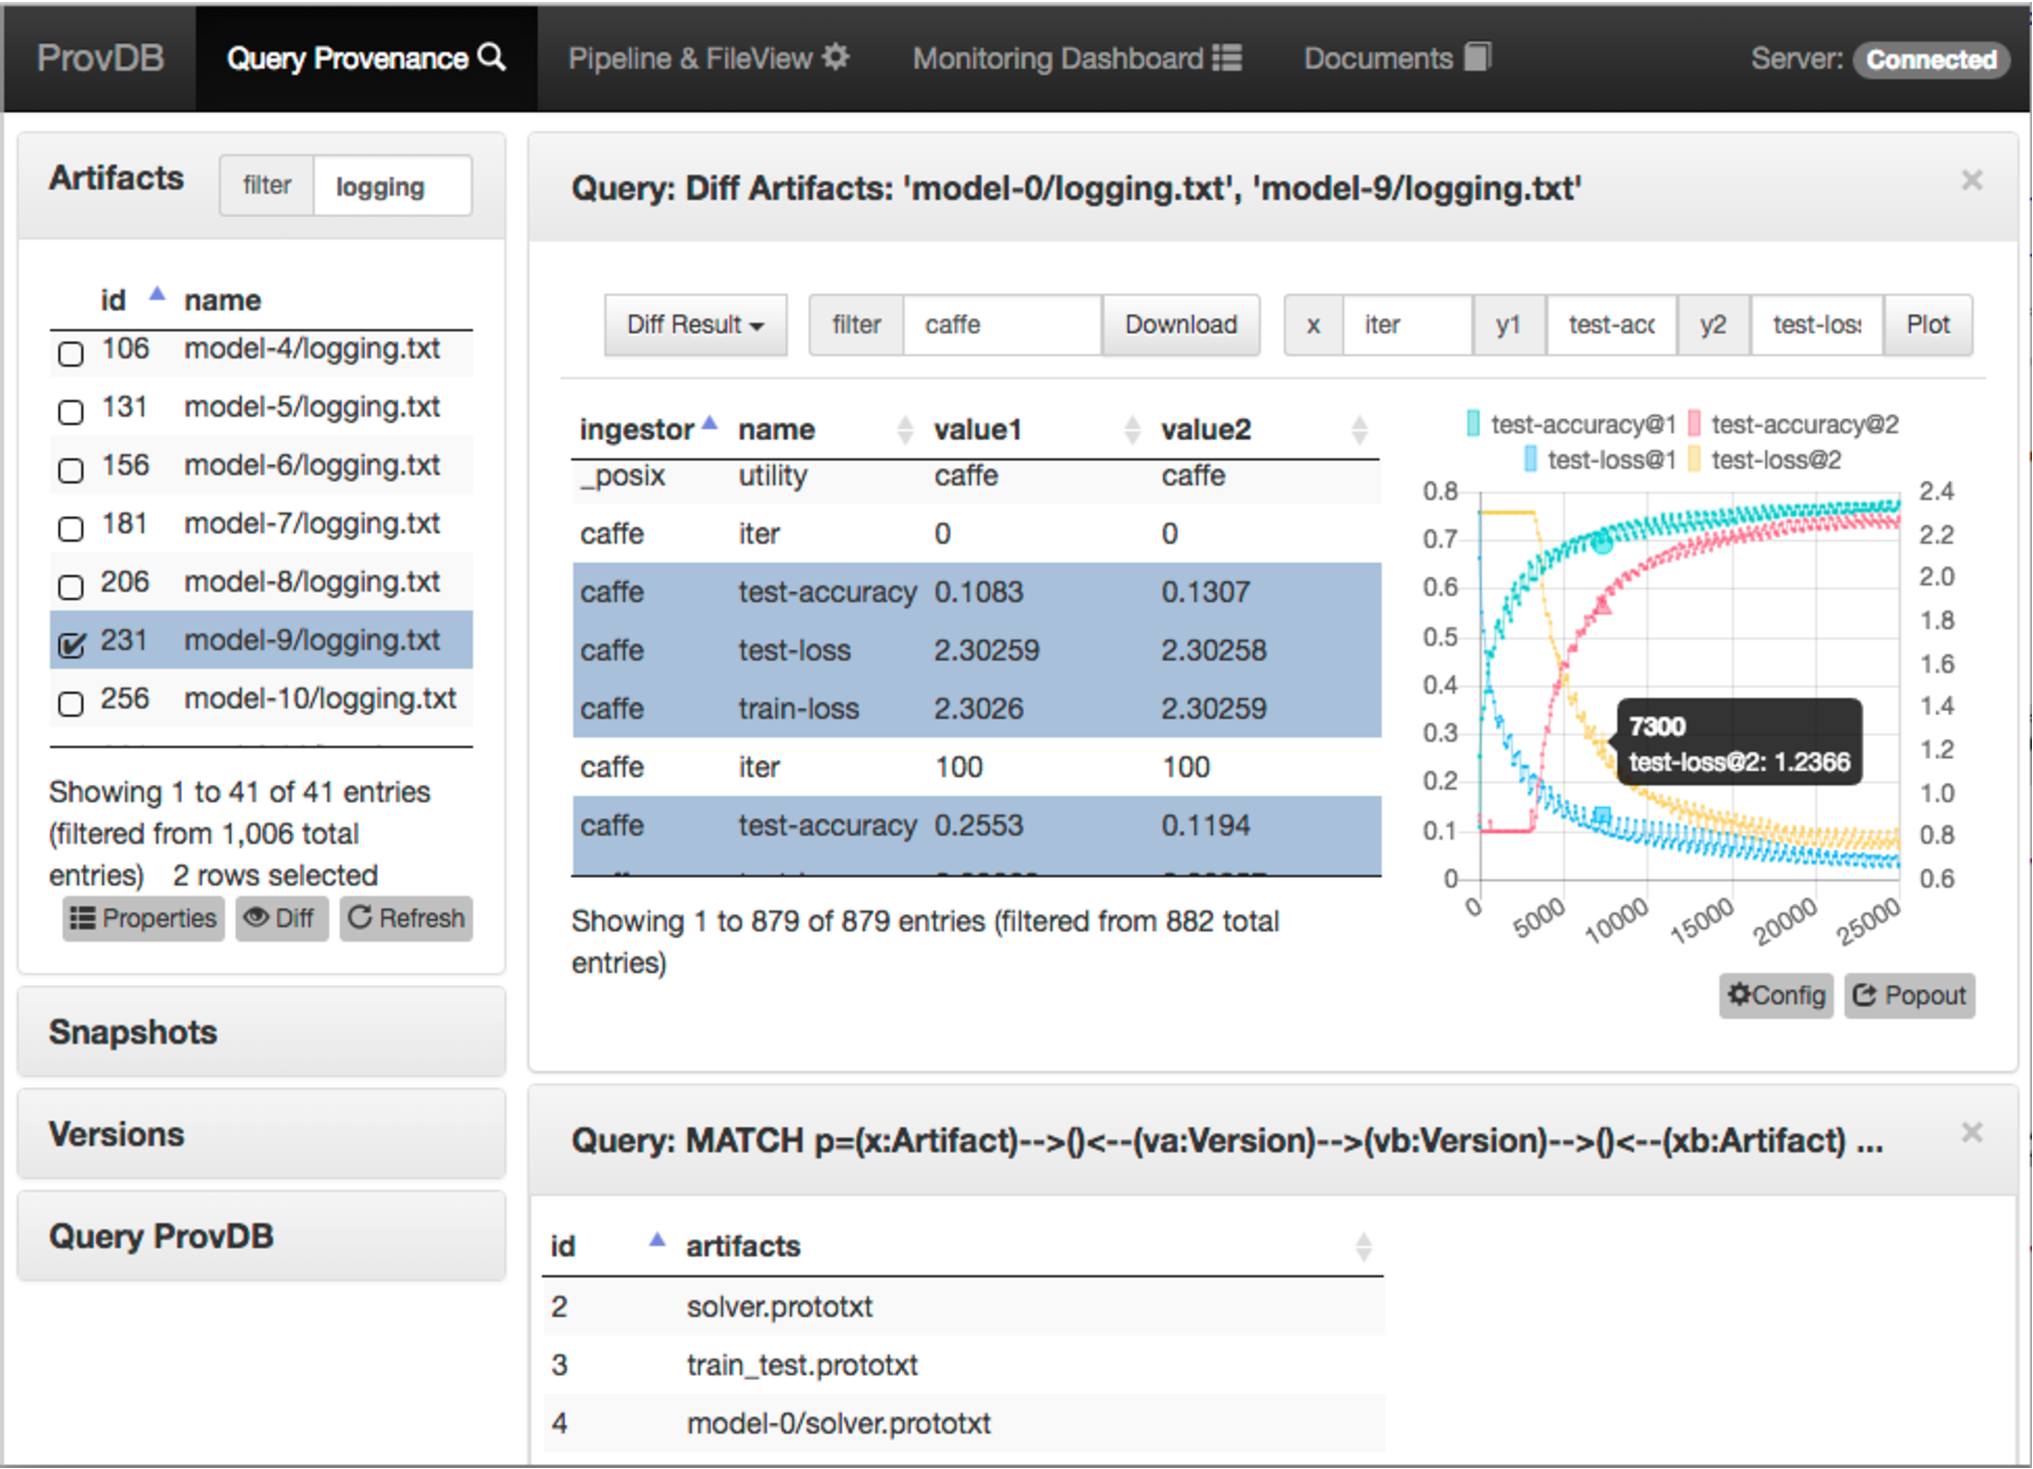
\includegraphics[width=0.46\textwidth]{figs/showcase_diff_nav.pdf}
  \label{fig:showcase_diff_nav}
}
~~
\subfigure[Cypher Query to Find Related Changes via Derivations]{
  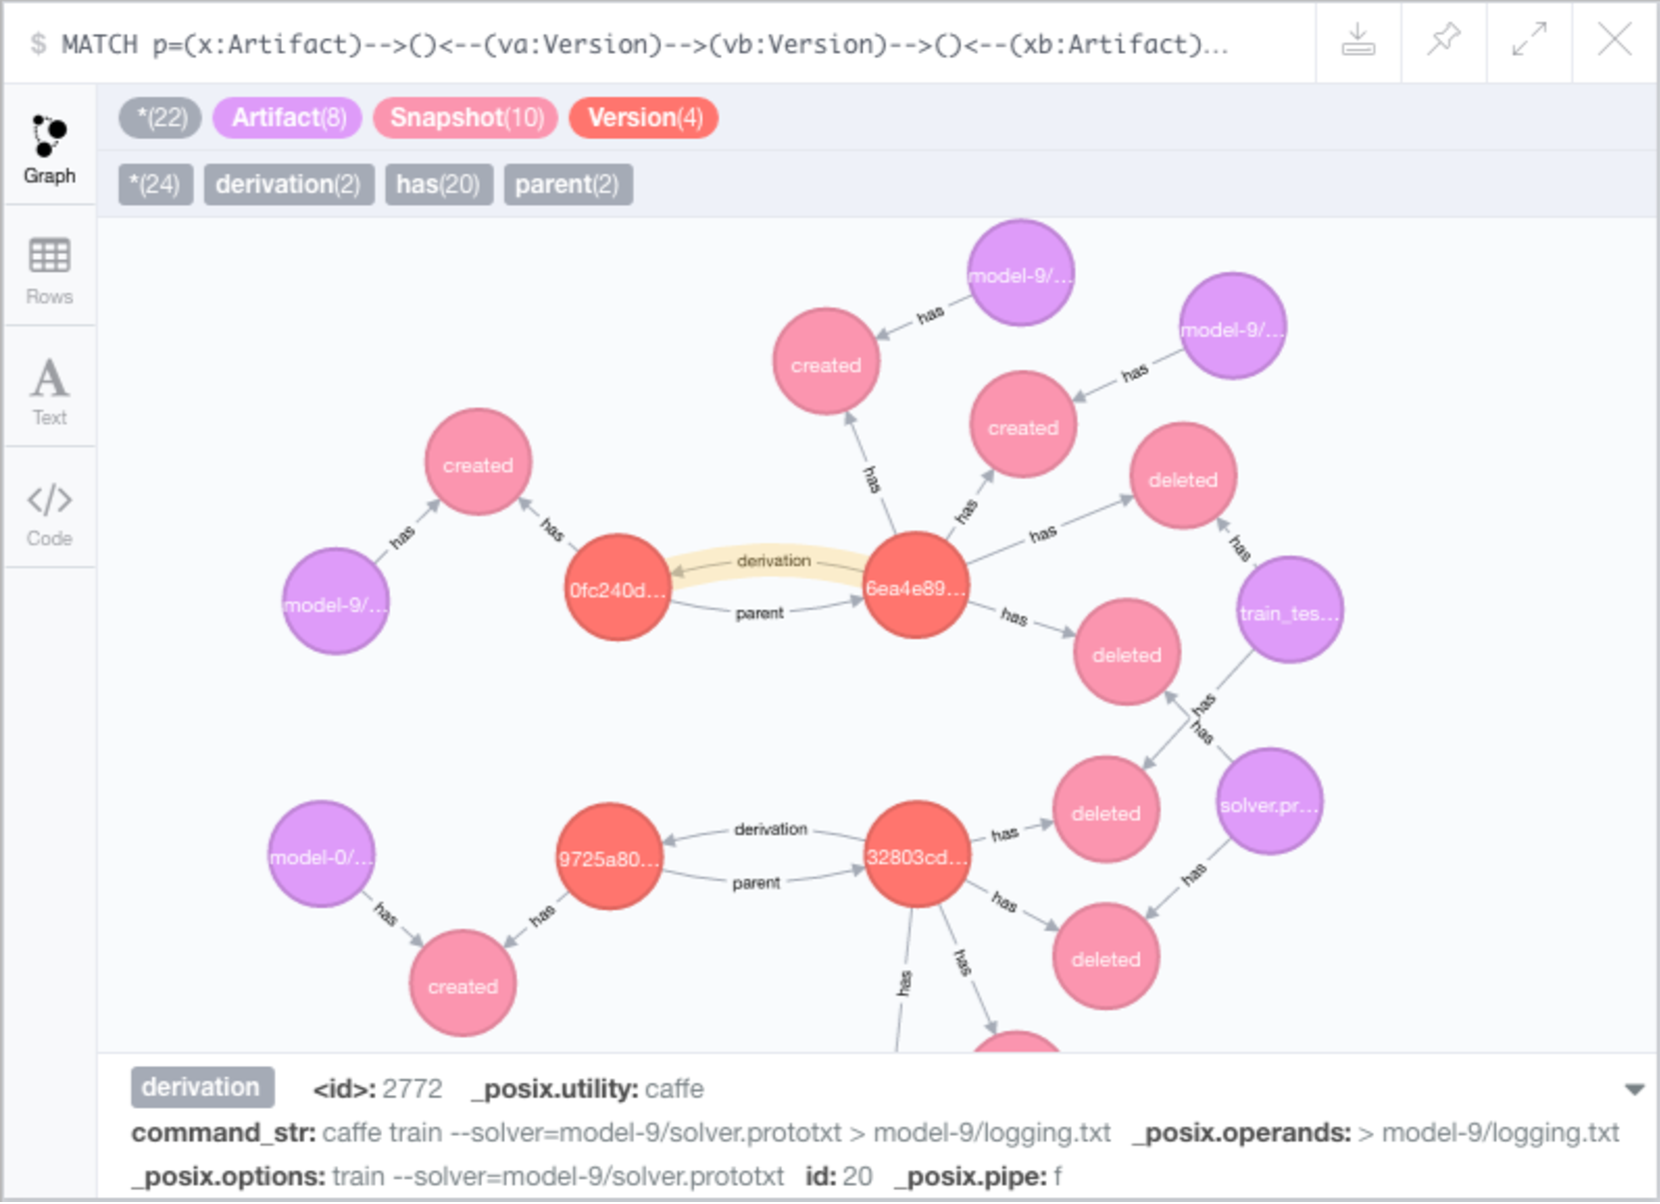
\includegraphics[width=0.46\textwidth]{figs/showcase_neo4j_nav.pdf}
  \label{fig:showcase_neo_nav}
}
}
\vspace{-10pt}
\caption{Illustration of \provdb interfaces}
\vspace{-10pt}
\label{fig:showcase}
\end{figure*}


Many such queries naturally result in one or more time series of values (e.g., properties of an artifact over time as it evolves, results of ``diff'' queries discussed below); \provdb supports a uniform visual interface for plotting such time series data, and comparing two different time series (see below for an example).


\topic{Illustrative Example:} Figure~\ref{fig:showcase} shows the \provdb Web GUI using a {\tt caffe} deep learning project. In this project, 41 deep neural networks are created for a face classification task. The user tries out models by editing and training models. In Fig~\ref{fig:showcase_diff_nav}, an introspection query asks how different are two trained models (\emph{model-0} and \emph{9}). Using the GUI, the user filters artifacts, and diffs their result logging files. In the right side query result pane, the ingested properties are diffed. The {\tt caffe} ingestor properties are numerical time series; using the provided charting tool, the user plots the training loss and accuracy against the iteration number. From the results, we can see that \emph{model-9} does not train well in the beginning, but ends up with similar accuracy. To understand why, a deep diff between the two can be issued in the GUI and complex Cypher queries can be used as well. In Fig.~\ref{fig:showcase_neo_nav}, the query finds previous derivations and shared snapshots, which are training config files; more introspection can be done by finding changed hyperparameters.


\begin{figure*}[t!]
\subfigure[Segmentation Query Examples]{
  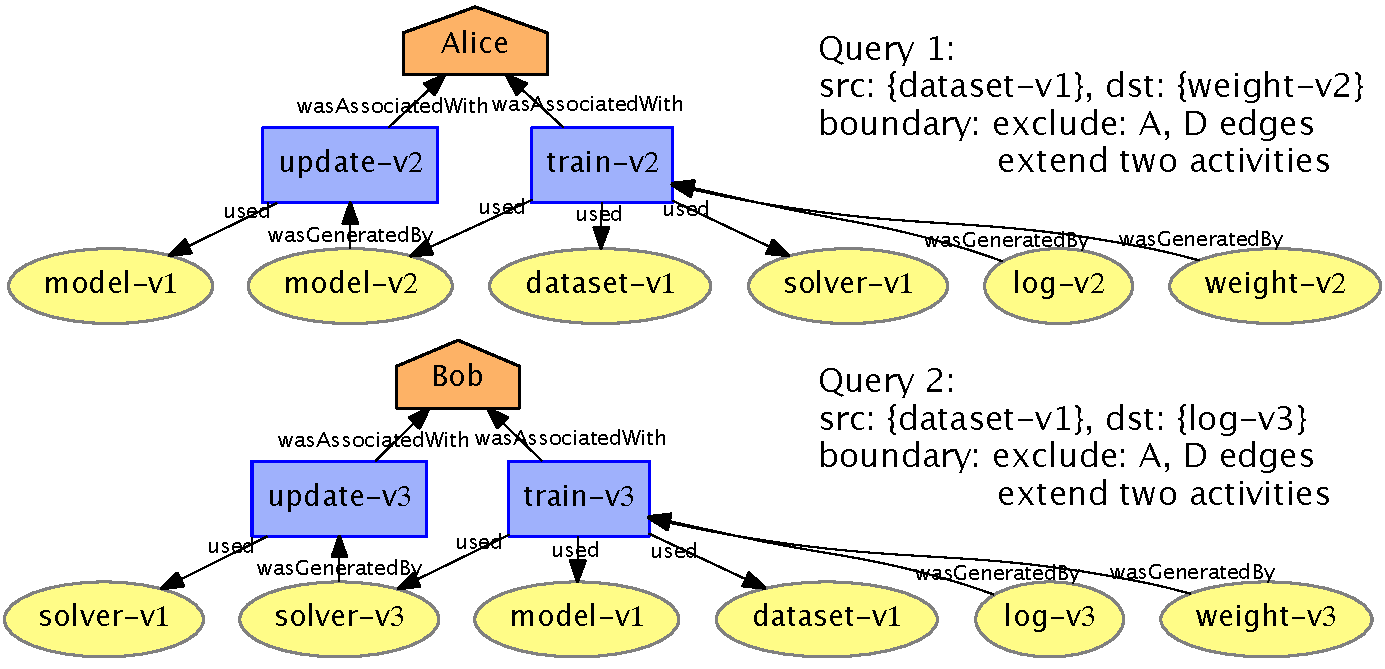
\includegraphics[width=0.475\textwidth,trim=0 0 0 12]{figs/query_example_seg_merged.pdf}
  \label{fig:example_query_segmentation}
}
\subfigure[Summarization Query Examples]{
  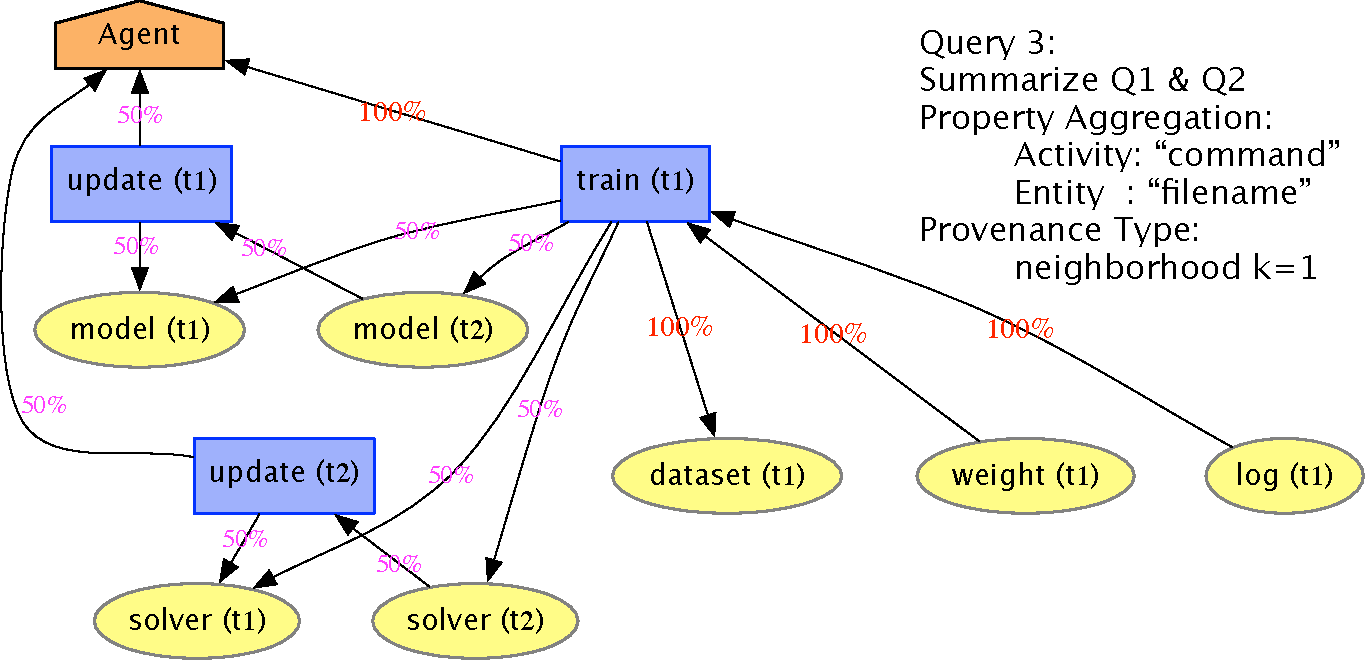
\includegraphics[width=0.48\textwidth,trim=0 0 0 12]{figs/query_example_sum_merged.pdf}
  \label{fig:example_query_summarization}
}
\vspace{-7pt}
\caption{Examples of Segmentation and Summarization Queries}
\vspace{-12pt}
\label{fig:example_queries}
\end{figure*}


\subsection{Graph Segmentation and Summarization Queries}
As discussed above, the extant graph query languages are not rich enough to support common provenance analysis queries. 
One of our goals with ongoing work is to initiate a more systematic study of
    abstract graph operators that modern graph databases need to support to be a viable option for storing provenance graphs. 
By observing the characteristics of the provenance graph in analytics lifecycle and identifying the requirements for the query facilities\eat{
(Sec.~\ref{subsec:datamodel})}, we propose two new graph operators as a starting point:


\topic{Segmentation:} A very important provenance query type of interest is querying ancestors and descendants of entities~\cite{freire2008provenance,pql_harvard@ipaw08}.
In our context, the users introspect the lifecycle and identify issues by analyzing dependencies among snapshots. Lack of a workflow
skeleton and clear boundaries makes the provenance query more difficult. Moreover the user may not be
able to specify all interested entities in a query due to partial knowledge. 
We propose a segmentation operator that takes sets of source and destination entities, and induces other important unknown entities 
satisfying a set of specified boundary criteria.

\vspace{-3pt}
\begin{example}
\label{exp:segop_q1_2}
In Fig.~\ref{fig:example_query_segmentation}, we show two examples of segmentation query. In Query 1 ($Q_1$), Bob was interested in what Alice did in version $v_2$. He did not know the details of activities and the entities Alice touched, instead he set \{\emph{dataset}\}, \{\emph{weight}\} as querying entities to see how the \emph{weight} in Alice's version $v_2$ was connected to the \emph{dataset}. He filtered out uninterested edge types (.e.g, \wasAttributedTo, \wasDerivedFrom) and excluded actions in earlier commits (e.g., $v_1$) by setting the boundaries as two activities away from those querying entities. \eat{In the figure, t}The system found connections among the querying entities, and included vertices within the boundaries. After interpreting the result, Bob knew Alice updated the model definitions in \emph{model}. On the other hand, Alice would understand how Bob improved the accuracy and learn from him. In Query 2 ($Q_2$), instead of learned \emph{weight}, accuracy property associated \emph{log} entity is used as querying entity along with \emph{dataset}. The result showed Bob only updated solver file. 
\end{example}

\topic{Summarization:} In workflow systems, querying the workflow skeleton (aka prospective provenance) is an important use case~\cite{bpql_milo@vldb06} and one of the {\em provenance challenges}~\cite{prov_challenges@website}. In our context, even though a static workflow skeleton is not present, summarizing a skeleton of similar processing pipelines, showing commonalities and identifying abnormal behaviors are very useful query capabilities. However, general graph summarization techniques~\cite{summary_tutorial@pvldb17} are not applicable to provenance graphs due to the subtle provenance meanings and constraints of the data model~\cite{prov_dm@w3c_tr13,provabs_pmissier@ipaw14,agg_lucmoreau@gam15}. 
Hence, we propose a summarization operator with multi-resolution capabilities for provenance graphs. 
It operates over query results of segmentation and allows tuning the summary by ignoring vertex details and characterizing local structures, and ensures provenance meaning through path constraints.


\vspace{-3pt}
\begin{example}
\label{exp:sumop_q3}
In Fig.~\ref{fig:example_query_summarization}, an outsider to the team (e.g., auditor, new team member) wanted to see the activity overview in the project. Segmentation queries (e.g., $Q_1$, $Q_2$ in Fig.~\ref{fig:example_query_segmentation}) only show individual trails of the analytics process at the snapshot level. The outsider issued a summarization query, Query 3 ($Q_3$), by specifying the aggregation over three types of vertices (viewing Alice and Bob as an abstract team member, ignoring details of files and activities), and defining the provenance meanings as a 1-hop neighborhood. The system merged $Q_1$ and $Q_2$ into a summary graph\eat{according to the query}. In Fig.~\ref{fig:example_query_summarization}, the vertices suffixed name with provenance types to show alternative generation process, while edges are labeled with their frequency of appearance among segments. The query issuer would vary the summary conditions at different resolutions.
\end{example}

\noindent
See~\cite{provquery_long} for a more in-depth discussion, including new query execution techniques for such queries.

\section{Related Work}
\label{sec:related}
There has been much work on scientific workflow systems over the years, with some of the prominent systems being Kepler\nosubcite{~\cite{ludascher2006scientific}},
Taverna\nosubcite{~\cite{oinn2006taverna}}, Galaxy\nosubcite{~\cite{giardine2005galaxy}}, iPlant\nosubcite{~\cite{goff2011iplant}},
VisTrails\nosubcite{~\cite{bavoil2005vistrails}}, Chimera\nosubcite{~\cite{foster2002chimera}}, Pegasus\nosubcite{~\cite{DBLP:journals/sp/DeelmanSSBGKMVBGLJK05}}, to name a 
few\footnote{We omit the citations for brevity; a more detailed discussion with citations can be found in~\cite{provdb@hilda17,provquery_long}}. 
These systems often center around creating, automating, and monitoring a well-defined workflow or data analysis pipeline. But they cannot easily handle fast-changing pipelines, and typically are not suitable for ad hoc collaborative data science workflows where clear established pipelines may not exist except in the final, stable versions. Moreover, these systems typically do not support the entire range of tools or systems that the users may want to use, they impose a high overhead on the user time and can substantially increase the development time, and often require using specific computational environment. Further, many of these systems require centralized storage and computation, which may not be an option for large datasets. 

Many users find {\bf version control systems} (e.g., {\tt git, svn}) and related hosted platforms (e.g., {\tt GitHub, GitLab}) more appropriate for their day-to-day
needs.  However, these systems are typically too ``low-level'', and don't support capturing higher-level workflows or provenance information. The versioning API
supported by these systems is based on a notion of files, and is not capable of allowing data researchers to reason about data contained within versions and the
relationships between the versions in a holistic manner. \provdb can be seen as providing rich introspection and querying capabilities those systems lack. 


Recently, there is emerging interest in developing systems for managing different aspects in the modeling lifecycle, such as building modeling lifecycle
platforms~\cite{google_tfx@kdd17}, accelerating iterative modeling process~\cite{columbus_tods16p}, managing developed models~\cite{modeldb_HILDA16p,modelhub@icde17},
organizing lifecycle provenance and metadata~\cite{ground@cidr17,provdb@hilda17,amazon_metadata@learningsys17},  auto-selecting
models~\cite{model_selection_arun_record15p}, hosting and discovering reference models~\cite{openml@kddexp13,discovery@deem17}, and assisting
collaboration~\cite{kandogan2015labbookp}.  Issues of querying evolving and verbose provenance effectively are typically not considered in that work.

There has also been much work on {\bf provenance}, with increasing interest in the recent years. The work in that space can be roughly categorized in two types: data
provenance (aka fine-granularity) and workflow provenance (aka coarse-granularity). Data provenance is discussed in dataflow systems, such as RDBMS, Pig Latin, and
Spark~\cite{survey_chiew@ftdb09,lipstick@pvldb11,titian@pvldb15}, while workflow provenance studies address complex interactions among high-level conceptual components
in various computational tasks, such as scientific workflows, business processes, and
cybersecurity~\cite{freire2008provenance,freire2008provenance,bpql_milo@vldb06,linuxprov_abates@atc15}.  Unlike retrospective query facilities in scientific workflow
provenance systems~\cite{freire2008provenance}, their processes are predefined in \emph{workflow skeletons}, and multiple executions generate different instance-level
provenance \emph{run graphs} and have clear boundaries. Taking advantages of the skeleton\eat{definition}, there are lines of research \eat{to aid}for advanced ancestry
query processing\eat{are important topics of study}, such as defining user views over such skeleton to aid queries on verbose run graphs~\cite{zoom_penn@icde08},
executing reachability query on the run graphs efficiently~\cite{reachability_optimallabeling_upenn@sigmod10}, storing run graphs generated by the skeletons
compactly~\cite{compression_bertram@edbt09}, and using visualization as examples to ease query construction~\cite{visualization@vis05}. 

Most relevant work is querying evolving script provenance~\cite{ingestions_noworkflow@ipaw14,noworkflow_evolution@ipaw16}. Because script executions form clear run graph
boundary, query facilities to visualize and difference execution run graphs are proposed. In our context, as there are no clear boundaries of run graphs, it is crucial
to design query facilities allowing the user to express the logical run graph segments and specify the boundary conditions first. Our method can also be applied on
script provenance by segmenting within and summarizing across evolving run graphs.


\section{Conclusion}
In this paper, we presented our approach to simplify lifecycle management of ad hoc, collaborative analysis workflows that are becoming prevalent in most application
domains today. Our system, \provdb, is based on the premise that a large amount of provenance and metadata information can be captured passively, and analyzing that
information in novel ways can immensely simplify the day-to-day processes undertaken by data analysts. Our initial experience with using this prototype for a deep
learning workflow (for a computer vision task) shows that even with limited functionality, it can simplify the bookkeeping tasks and make it easy to compare the effects
of different hyperparameters and neural network structures. However, many interesting and hard systems and conceptual challenges remain to be addressed in capturing and
exploiting such information to its fullest extent. In particular, there are many potential ways to use the rich provenance and context metadata that \provdb collects to
answer explanation queries to understand the origins of a piece of data or introspection queries to identify practices like {\em p-value hacking}. Continuous monitoring
of this data can also help identify issues during deployment of data science pipelines (e.g., {\em concept drifts}). In addition, the large volumes of versioned
provenance information requires development of new graph data management systems, including new graph query operators, that we are actively investigating in ongoing
work.


\begin{thebibliography}{10}

\bibitem{prov_challenges@website}
{Provenance Challenge}.
\newblock \url{http://twiki.ipaw.info}.
\newblock Accessed: 2017-07.

\bibitem{prov_segmentation@tapp16}
R.~Abreu, D.~Archer, E.~Chapman, J.~Cheney, H.~Eldardiry, and A.~Gasc{\'o}n.
\newblock Provenance segmentation.
\newblock In {\em 8th Workshop on the Theory and Practice of Provenance
  (TaPP)}, 2016.

\bibitem{lipstick@pvldb11}
Y.~Amsterdamer, S.~B. Davidson, D.~Deutch, T.~Milo, J.~Stoyanovich, and
  V.~Tannen.
\newblock Putting lipstick on pig: Enabling database-style workflow provenance.
\newblock {\em {PVLDB}}, 5(4):346--357, 2011.

\bibitem{bertram_lang@edbt10}
M.~K. Anand, S.~Bowers, and B.~Lud{\"{a}}scher.
\newblock Techniques for efficiently querying scientific workflow provenance
  graphs.
\newblock In {\em {EDBT}}, 2010.

\bibitem{compression_bertram@edbt09}
M.~K. Anand, S.~Bowers, T.~M. McPhillips, and B.~Lud{\"{a}}scher.
\newblock Efficient provenance storage over nested data collections.
\newblock In {\em {EDBT}}, 2009.

\bibitem{survey_querylang@arix16}
R.~Angles, M.~Arenas, P.~Barcel{\'{o}}, A.~Hogan, J.~L. Reutter, and D.~Vrgoc.
\newblock Foundations of modern query languages for graph databases.
\newblock {\em ACM Computing Surveys}, 50(5):68:1--68:40, 2017.

\bibitem{gquery_theory@pods13}
P.~B. Baeza.
\newblock Querying graph databases.
\newblock In {\em PODS}, 2013.

\bibitem{reachability_optimallabeling_upenn@sigmod10}
Z.~Bao, S.~B. Davidson, S.~Khanna, and S.~Roy.
\newblock An optimal labeling scheme for workflow provenance using skeleton
  labels.
\newblock In {\em SIGMOD}, 2010.

\bibitem{linuxprov_abates@atc15}
A.~M. Bates, D.~Tian, K.~R.~B. Butler, and T.~Moyer.
\newblock Trustworthy whole-system provenance for the linux kernel.
\newblock In {\em 24th {USENIX} Security Symposium}, 2015.

\bibitem{visualization@vis05}
L.~Bavoil, S.~P. Callahan, C.~E. Scheidegger, H.~T. Vo, P.~Crossno, C.~T.
  Silva, and J.~Freire.
\newblock Vistrails: Enabling interactive multiple-view visualizations.
\newblock In {\em 16th {IEEE} Visualization Conference (VIS)}, 2005.

\bibitem{google_tfx@kdd17}
D.~Baylor et al. 
\newblock {TFX:} {A} tensorflow-based production-scale machine learning
  platform.
\newblock In {\em KDD}, 2017.

\bibitem{bpql_milo@vldb06}
C.~Beeri, A.~Eyal, S.~Kamenkovich, and T.~Milo.
\newblock Querying business processes.
\newblock In {\em VLDB}, 2006.

\bibitem{datahub2015}
A.~P. Bhardwaj, S.~Bhattacherjee, A.~Chavan, A.~Deshpande, A.~Elmore,
  S.~Madden, and A.~Parameswaran.
\newblock {DataHub: Collaborative Data Science {\&} Dataset Version Management
  at Scale}.
\newblock {\em CIDR}, 2015.

\bibitem{dataset2015}
S.~Bhattacherjee, A.~Chavan, S.~Huang, A.~Deshpande, and A.~Parameswaran.
\newblock {Principles of Dataset Versioning: Exploring the Recreation/Storage
  Tradeoff}.
\newblock {\em PVLDB}, 2015.

\bibitem{rstore}
S.~Bhattacherjee, A.~Deshpande.
\newblock Storing and querying versioned documents in the cloud.
\newblock In {\em {ICDE}}, 2018.

\bibitem{zoom_penn@icde08}
O.~Biton, S.~C. Boulakia, S.~B. Davidson, and C.~S. Hara.
\newblock Querying and managing provenance through user views in scientific
  workflows.
\newblock In {\em ICDE}, 2008.

\bibitem{dex@sigmod17}
A.~Chavan and A.~Deshpande.
\newblock {DEX:} query execution in a delta-based storage system.
\newblock In {\em SIGMOD}, 2017.

\bibitem{provenance2015}
A.~Chavan, S.~Huang, A.~Deshpande, A.~Elmore, S.~Madden, and A.~Parameswaran.
\newblock {Towards a Unified Query Language for Provenance and Versioning}.
\newblock {\em Theory and Practice of Provenance {(TaPP)}}, 2015.

\bibitem{survey_chiew@ftdb09}
J.~Cheney, L.~Chiticariu, and W.~C. Tan.
\newblock Provenance in databases: Why, how, and where.
\newblock {\em FnT}, 2009.

\bibitem{freire2008provenance}
J.~Freire, D.~Koop, E.~Santos, and C.~T. Silva.
\newblock Provenance for computational tasks: A survey.
\newblock {\em Computing in Science \& Engineering}, 2008.

\bibitem{ground@cidr17}
J.~M. Hellerstein, V.~Sreekanti, J.~E. Gonzalez, J.~Dalton, A.~Dey, S.~Nag,
  K.~Ramachandran, S.~Arora, A.~Bhattacharyya, S.~Das, M.~Donsky, G.~Fierro,
  C.~She, C.~Steinbach, V.~Subramanian, and E.~Sun.
\newblock Ground: {A} data context service.
\newblock In {\em {CIDR}}, 2017.

\bibitem{pql_harvard@ipaw08}
D.~A. Holland, U.~J. Braun, D.~Maclean, K.-K. Muniswamy-Reddy, and M.~I.
  Seltzer.
\newblock Choosing a data model and query language for provenance.
\newblock In {\em Intl. Provenance and Annotation Workshop (IPAW)}, 2010.

\bibitem{titian@pvldb15}
M.~Interlandi, K.~Shah, S.~D. Tetali, M.~A. Gulzar, S.~Yoo, M.~Kim, T.~D.
  Millstein, and T.~Condie.
\newblock Titian: Data provenance support in spark.
\newblock {\em {PVLDB}}, 9(3):216--227, 2015.

\bibitem{kandogan2015labbookp}
E.~Kandogan, M.~Roth, P.~M. Schwarz, J.~Hui, I.~Terrizzano, C.~Christodoulakis,
  and R.~J. Miller.
\newblock Labbook: Metadata-driven social collaborative data analysis.
\newblock In {\em {IEEE} International Conference on Big Data}, 2015.

\bibitem{katz1990toward}
R.~H. Katz.
\newblock {Toward a unified framework for version modeling in engineering
  databases}.
\newblock {\em ACM Computing Surveys (CSUR)}, 22(4):375--409, 1990.

\bibitem{summary_tutorial@pvldb17}
A.~Khan, S.~S. Bhowmick, and F.~Bonchi.
\newblock Summarizing static and dynamic big graphs.
\newblock {\em {PVLDB}}, 2017.

\bibitem{model_selection_arun_record15p}
A.~Kumar, R.~McCann, J.~F. Naughton, and J.~M. Patel.
\newblock Model selection management systems: The next frontier of advanced
  analytics.
\newblock {\em {SIGMOD} Record}, 44(4):17--22, 2015.

\bibitem{decibel}
M.~Maddox, D.~Goehring, A.~J. Elmore, S.~Madden, A.~G. Parameswaran, and
  A.~Deshpande.
\newblock Decibel: The relational dataset branching system.
\newblock {\em {PVLDB}}, 9(9):624--635, 2016.

\bibitem{dda_microsoft@cidr17}
R.~Mavlyutov, C.~Curino, B.~Asipov, and P.~Cudr{\'{e}}{-}Mauroux.
\newblock Dependency-driven analytics: {A} compass for uncharted data oceans.
\newblock In {\em {CIDR}}, 2017.

\bibitem{provdb@hilda17}
H.~Miao, A.~Chavan, and A.~Deshpande.
\newblock {ProvDB:} lifecycle management of collaborative analysis workflows.
\newblock In {\em 2nd Workshop on Human-In-the-Loop Data Analytics,
  HILDA@SIGMOD}, 2017.

\bibitem{provquery_long}
H.~Miao and A.~Deshpande.
\newblock Understanding data science lifecycle provenance via graph
  segmentation and summarization.
\newblock CoRR abs/1810.04599, 2018.

\bibitem{discovery@deem17}
H.~Miao, A.~Li, L.~S. Davis, and A.~Deshpande.
\newblock On model discovery for hosted data science projects.
\newblock In {\em Workshop on Data Management for End-To-End Machine Learning,
  DEEM@SIGMOD}, 2017.

\bibitem{modelhub@icde17}
H.~Miao, A.~Li, L.~S. Davis, and A.~Deshpande.
\newblock Towards unified data and lifecycle management for deep learning.
\newblock In {\em ICDE}, 2017.

\bibitem{provabs_pmissier@ipaw14}
P.~Missier, J.~Bryans, C.~Gamble, V.~Curcin, and R.~D{\'{a}}nger.
\newblock {ProvAbs}: Model, policy, and tooling for abstracting {PROV} graphs.
\newblock In {\em Intl. Provenance and Annotation Workshop (IPAW)}, 2014.

\bibitem{prov_dm@w3c_tr13}
P.~Missier and L.~Moreau.
\newblock {PROV}-dm: The {PROV} data model.
\newblock {W3C} recommendation, W3C, 2013.
\newblock http://www.w3.org/TR/2013/REC-prov-dm-20130430/.

\bibitem{agg_lucmoreau@gam15}
L.~Moreau.
\newblock Aggregation by provenance types: {A} technique for summarising
  provenance graphs.
\newblock In {\em Proceedings Graphs as Models, GaM@ETAPS 2015, London, UK,
  11-12 April 2015.}, pages 129--144, 2015.

\bibitem{prov_stack@w3c_tr13}
L.~Moreau and P.~Groth.
\newblock {PROV}-overview.
\newblock {W3C} note, W3C, 2013.
\newblock http://www.w3.org/TR/2013/NOTE-prov-overview-20130430/.

\bibitem{pass_harvard@atc06}
K.~Muniswamy{-}Reddy, D.~A. Holland, U.~Braun, and M.~I. Seltzer.
\newblock Provenance-aware storage systems.
\newblock In {\em Proceedings of the 2006 {USENIX} Annual Technical Conference}, 2006.

\bibitem{ingestions_noworkflow@ipaw14}
L.~Murta, V.~Braganholo, F.~Chirigati, D.~Koop, and J.~Freire.
\newblock noworkflow: Capturing and analyzing provenance of scripts.
\newblock In {\em  International Provenance and Annotation Workshop (IPAW)}, 2014.

\bibitem{noworkflow_evolution@ipaw16}
J.~F. Pimentel, J.~Freire, V.~Braganholo, and L.~Murta.
\newblock Tracking and analyzing the evolution of provenance from scripts.
\newblock In {\em  International Provenance and Annotation Workshop (IPAW)}, 2016.

\bibitem{amazon_metadata@learningsys17}
S.~Schelter, J.~Boese, J.~Kirschnick, T.~Klein, and S.~Seufert.
\newblock Automatically tracking metadata and provenance of machine learning
  experiments.
\newblock In {\em NIPS Workshop on ML Systems (LearningSys)}, 2017.

\bibitem{pgql_oracle@grades16}
O.~van Rest, S.~Hong, J.~Kim, X.~Meng, and H.~Chafi.
\newblock {PGQL:} a property graph query language.
\newblock In {\em Proc. of the Intl. Workshop on Graph
  Data Management Experiences and Systems (GRADES)}, 2016.

\bibitem{openml@kddexp13}
J.~Vanschoren, J.~N. van Rijn, B.~Bischl, and L.~Torgo.
\newblock Openml: networked science in machine learning.
\newblock {\em {SIGKDD} Explorations}, 15(2):49--60, 2013.

\bibitem{modeldb_HILDA16p}
M.~Vartak, H.~Subramanyam, W.-E. Lee, S.~Viswanathan, S.~Husnoo, S.~Madden, and
  M.~Zaharia.
\newblock {ModelDB}: a system for machine learning model management.
\newblock In {\em Workshop on Human-In-the-Loop Data Analytics,
  HILDA@SIGMOD}, 2016.

\bibitem{columbus_tods16p}
C.~Zhang, A.~Kumar, and C.~R{\'e}.
\newblock Materialization optimizations for feature selection workloads.
\newblock {\em ACM Transactions on Database Systems (TODS)}, 41(1):2, 2016.

\end{thebibliography}

\end{document}
